\documentclass[a4paper,11pt]{article}

\usepackage[french]{babel}
\usepackage[utf8]{inputenc}
\usepackage[T1]{fontenc}
\usepackage[margin=2.2cm]{geometry}
\usepackage{graphicx}
\usepackage{booktabs}
\usepackage{enumitem}
\usepackage{xcolor}
\usepackage[colorlinks=true,linkcolor=blue!50!black,urlcolor=blue!50!black]{hyperref}
\usepackage{float}

\setlist{leftmargin=1.5em,itemsep=2pt,topsep=4pt}

\title{\textbf{Cahier des charges (version courte)} \\[4pt] \Large Puissance 4 RL}
\author{Loïc Lavorel}
\date{Semestre de printemps 2026 --- Advanced Mobile Applications (HES-SO)}

\begin{document}

\maketitle

\begin{center}
\textit{Repo : \url{https://github.com/loiclavorelM/puissance4}}
\end{center}

\section{Contexte et objectif}

Application mobile \textbf{Flutter} de Puissance 4, avec un backend
\textbf{100\,\% Serverpod} (Dart, PostgreSQL, authentification native), réalisée pour le
cours Advanced Mobile Applications et le Serverpod Hackathon (sept.--oct. 2026).
L'application doit être \textit{context-aware} et utiliser au moins un capteur.

Le joueur peut s'authentifier, gérer son profil, affronter un bot entraîné par
\textbf{apprentissage par renforcement} (3 niveaux), jouer contre un autre joueur en
ligne, progresser dans un classement \textbf{Elo} et revoir ses parties.

\section{Fonctionnalités}

\paragraph{Modes de jeu} (tous affichés par un \textbf{écran de jeu unique}) :
\begin{itemize}
  \item \textbf{Normal} --- contre un bot sur le téléphone, niveau au choix
        (Débutant, Medium, Expert). Jouable hors-ligne, sans effet sur l'Elo.
  \item \textbf{Classé} --- contre un bot \textbf{joué par le serveur}, choisi selon
        l'Elo du joueur. Le serveur valide chaque coup : le résultat ne peut pas être
        falsifié. Elo mis à jour en fin de partie.
  \item \textbf{Multijoueur} \textit{(optionnel)} --- 1 contre 1 en temps réel via un
        code de salle de 6 caractères (streams Serverpod). Sans effet sur l'Elo.
  \item \textbf{Replay} --- toute partie terminée peut être revue coup par coup depuis
        l'historique.
\end{itemize}

\paragraph{Compte et données.}
\begin{itemize}
  \item Authentification native Serverpod : email/mot de passe, Google ou invité
        (session anonyme).
  \item Profil (pseudo, photo prise avec la \textbf{caméra}, Elo), classement global
        par Elo et historique des parties.
  \item \textbf{Hors-ligne} \textit{(optionnel)} : les parties Normales sont stockées
        dans une base SQLite locale et synchronisées automatiquement avec le serveur
        au retour du réseau (\texttt{serverpod\_offline\_sync}).
\end{itemize}

\paragraph{Capteurs (context-aware).}
\begin{itemize}
  \item \textbf{Secousse} (accéléromètre) : réinitialise la partie, en mode Normal
        uniquement.
  \item \textbf{Téléphone posé à plat} : met automatiquement la partie Normale en pause.
  \item \textbf{Caméra} : photo de profil.
\end{itemize}

\paragraph{Règles des parties serveur (Classé et Multijoueur).} 60 s maximum par coup,
15 s pour revenir après une déconnexion. Une partie quittée avant tout coup du joueur
est annulée (sans effet sur l'historique ni l'Elo) ; sinon l'adversaire gagne.

\section{Système Elo}

Formule classique : $E = 1 / (1 + 10^{(Elo_{bot} - Elo_{joueur})/400})$, puis
$Elo' = Elo + K(S - E)$ avec $K = 32$ et $S \in \{1;\,0.5;\,0\}$.
Elo initial : 1000. Bots : Débutant 800, Medium 1200, Expert 1600.
Choix du bot en Classé : Elo $< 1000$ $\rightarrow$ Débutant, $< 1400$ $\rightarrow$
Medium, sinon Expert.

\section{Architecture}

\begin{itemize}
  \item \textbf{Flutter} : MVVM organisé par fonctionnalité
        (\texttt{features/<feature>/\{model,view,viewmodel\}}), Riverpod.
  \item \textbf{Serverpod} : un groupe d'endpoints par fonctionnalité, PostgreSQL comme
        source de vérité, streams pour le temps réel.
  \item \textbf{Paquet partagé} \texttt{puissance4\_rules} : règles du jeu et bot,
        utilisés à l'identique par l'app et le serveur.
  \item \textbf{IA} : modèles RL entraînés sur Google Colab, exportés en TFLite/ONNX et
        exécutés sur l'appareil ; en attendant, un bot heuristique les remplace.
\end{itemize}

\section{Maquettes}

\begin{figure}[H]
\centering
\begin{minipage}{0.24\textwidth}\centering
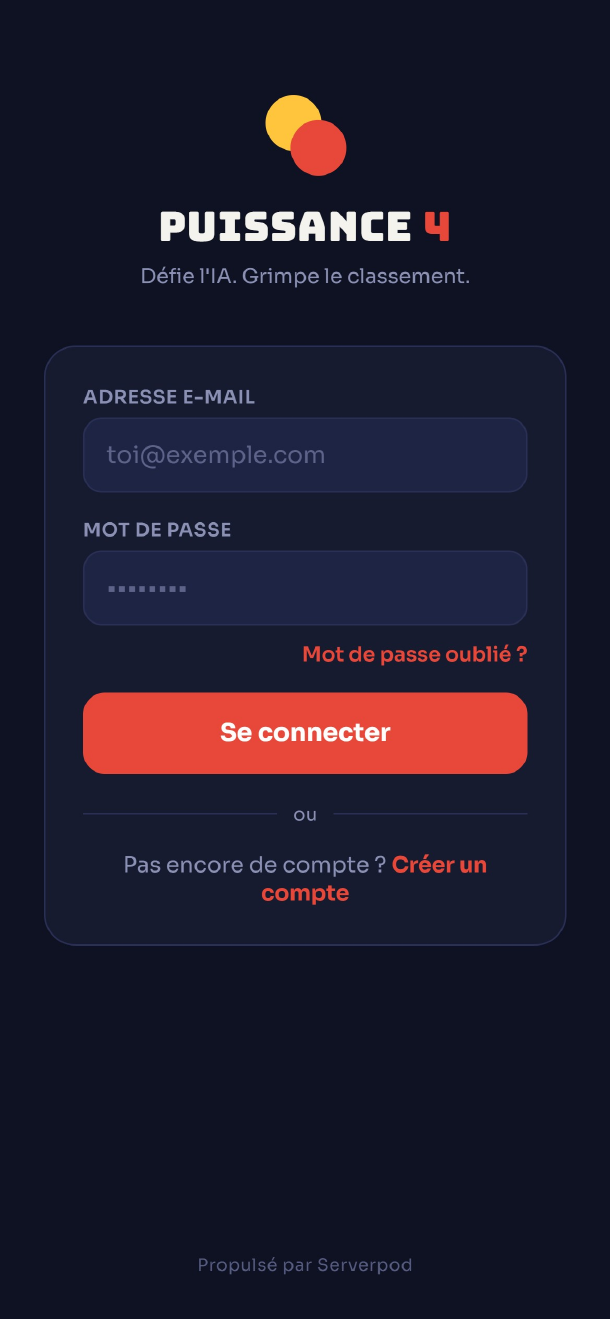
\includegraphics[width=\linewidth]{figures/maquette-1.png}\\[2pt]
\footnotesize (a) Connexion
\end{minipage}\hfill
\begin{minipage}{0.24\textwidth}\centering
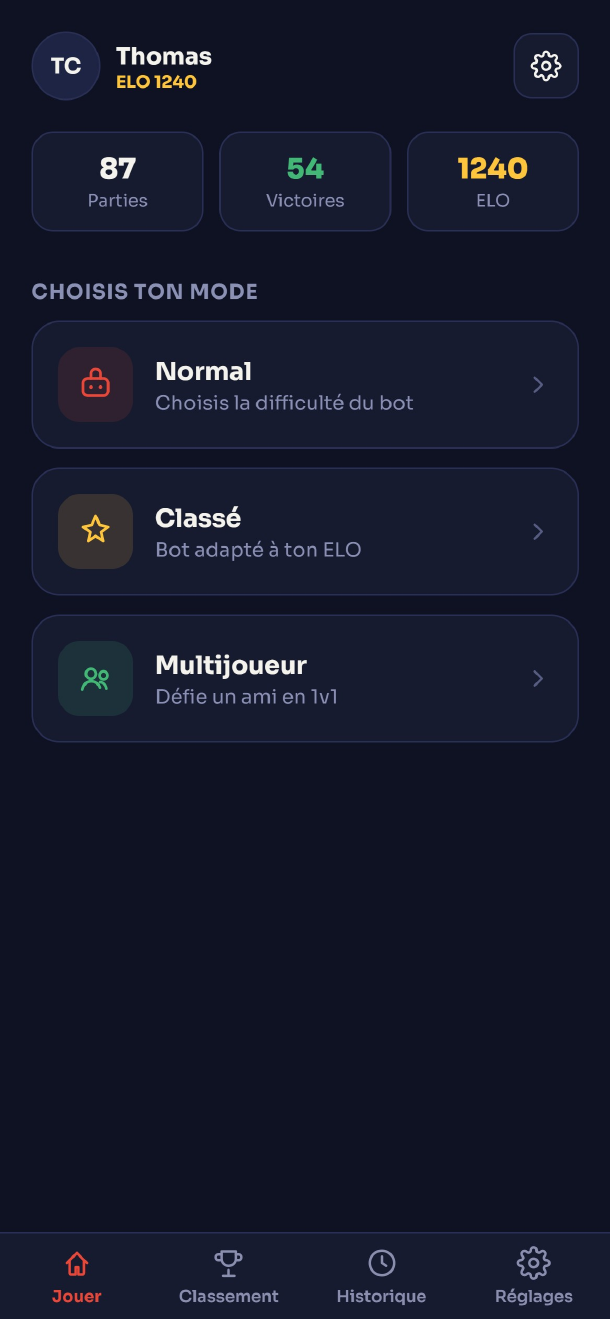
\includegraphics[width=\linewidth]{figures/maquette-2.png}\\[2pt]
\footnotesize (b) Accueil
\end{minipage}\hfill
\begin{minipage}{0.24\textwidth}\centering
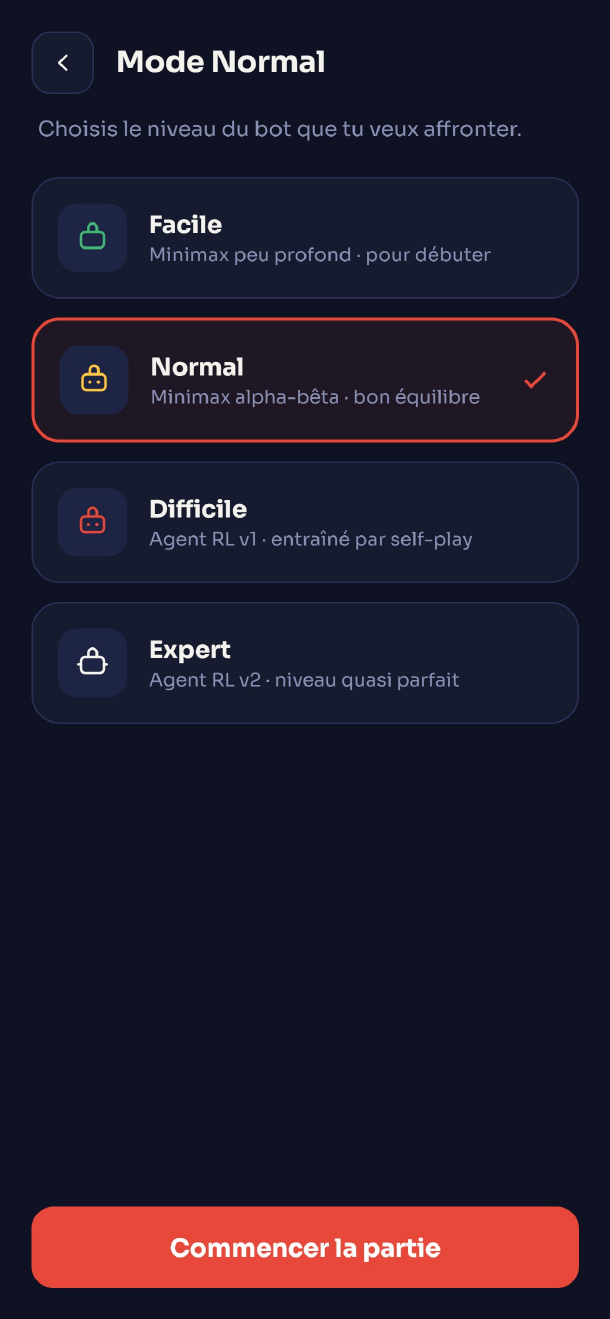
\includegraphics[width=\linewidth]{figures/maquette-3.png}\\[2pt]
\footnotesize (c) Choix du niveau
\end{minipage}\hfill
\begin{minipage}{0.24\textwidth}\centering
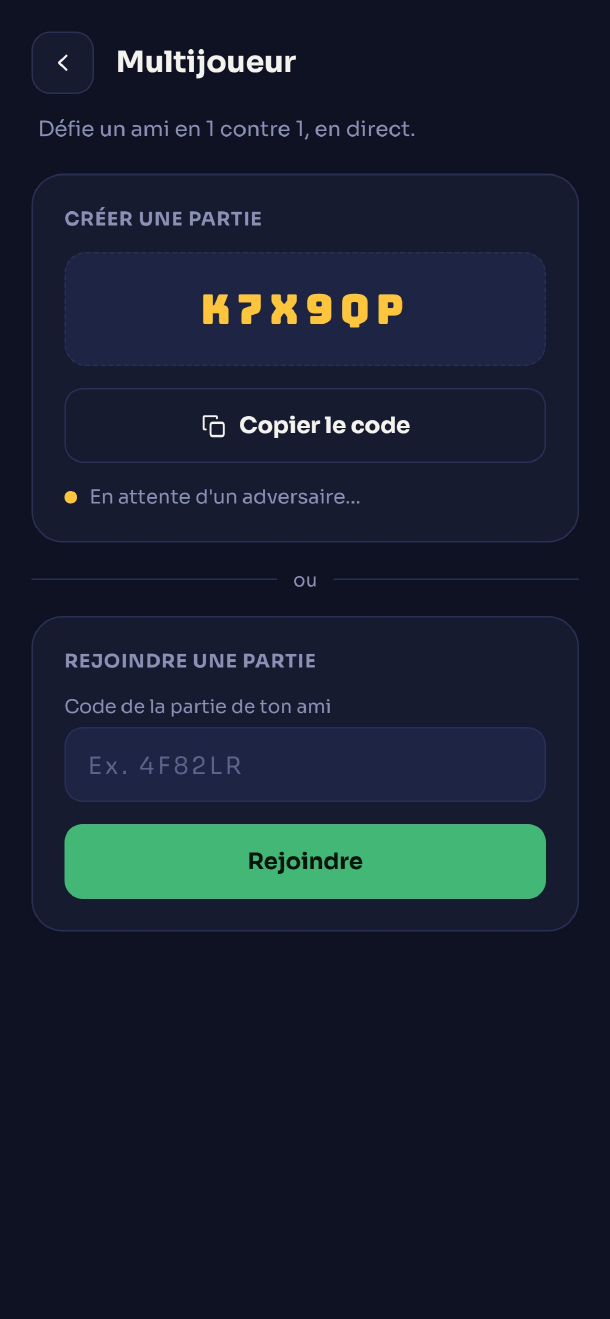
\includegraphics[width=\linewidth]{figures/maquette-4.png}\\[2pt]
\footnotesize (d) Multijoueur
\end{minipage}

\vspace{4mm}

\begin{minipage}{0.24\textwidth}\centering
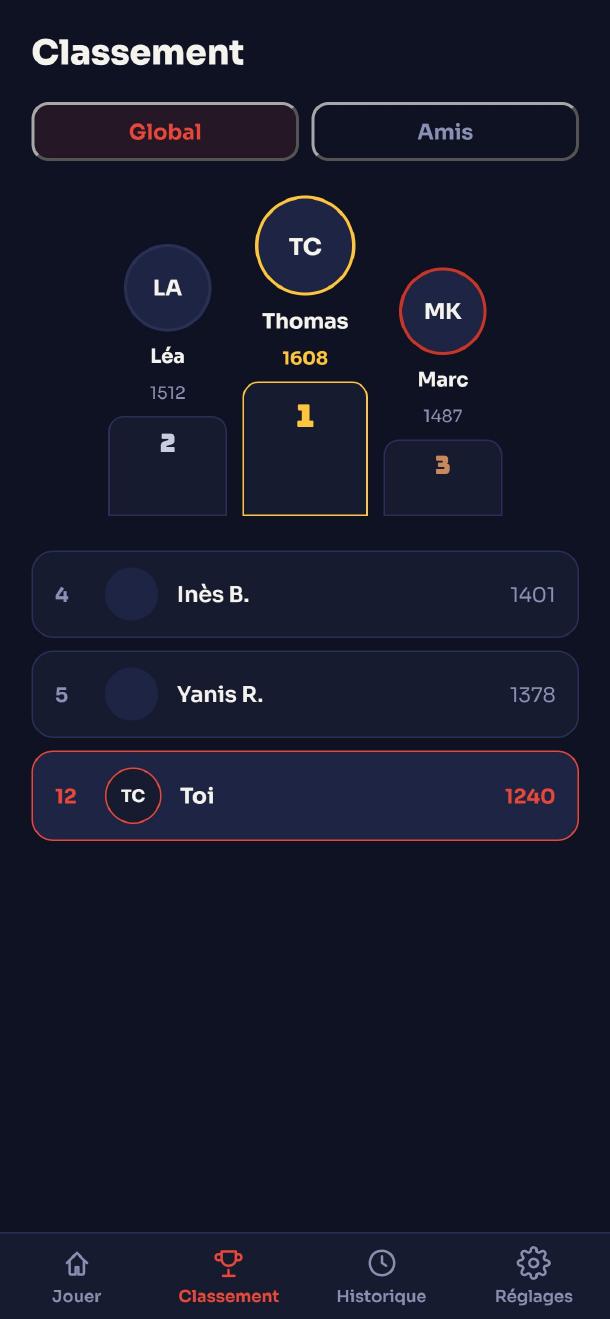
\includegraphics[width=\linewidth]{figures/maquette-5.png}\\[2pt]
\footnotesize (e) Classement
\end{minipage}\hspace{0.013\textwidth}
\begin{minipage}{0.24\textwidth}\centering
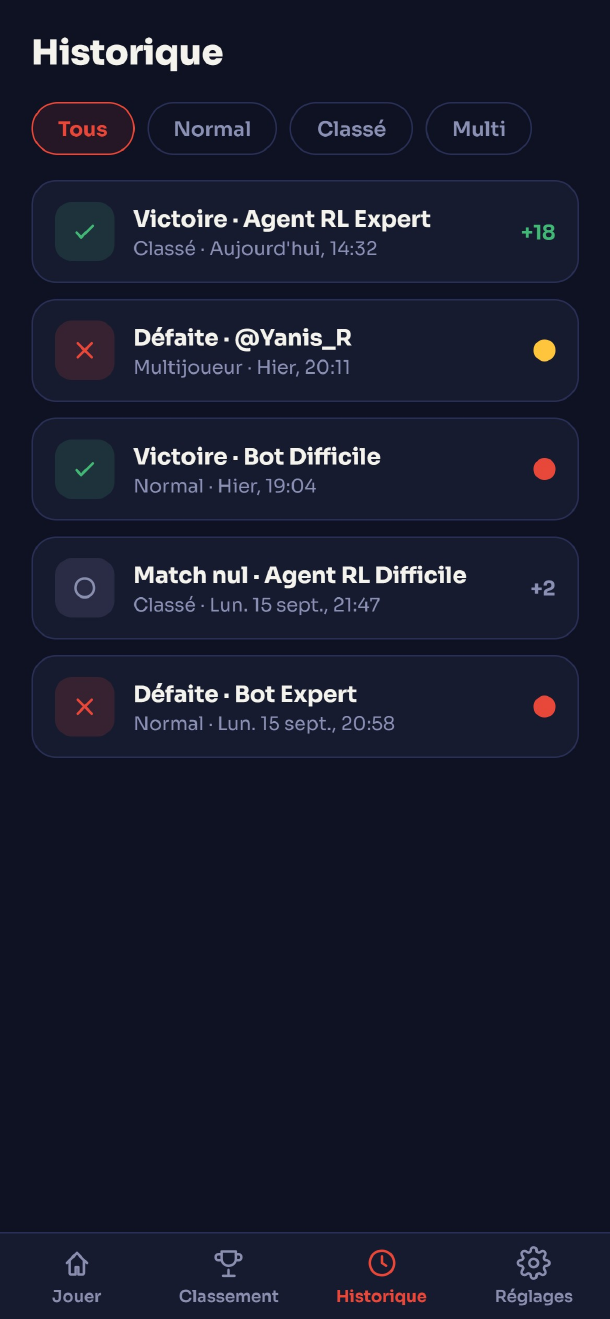
\includegraphics[width=\linewidth]{figures/maquette-6.png}\\[2pt]
\footnotesize (f) Historique
\end{minipage}\hspace{0.013\textwidth}
\begin{minipage}{0.24\textwidth}\centering
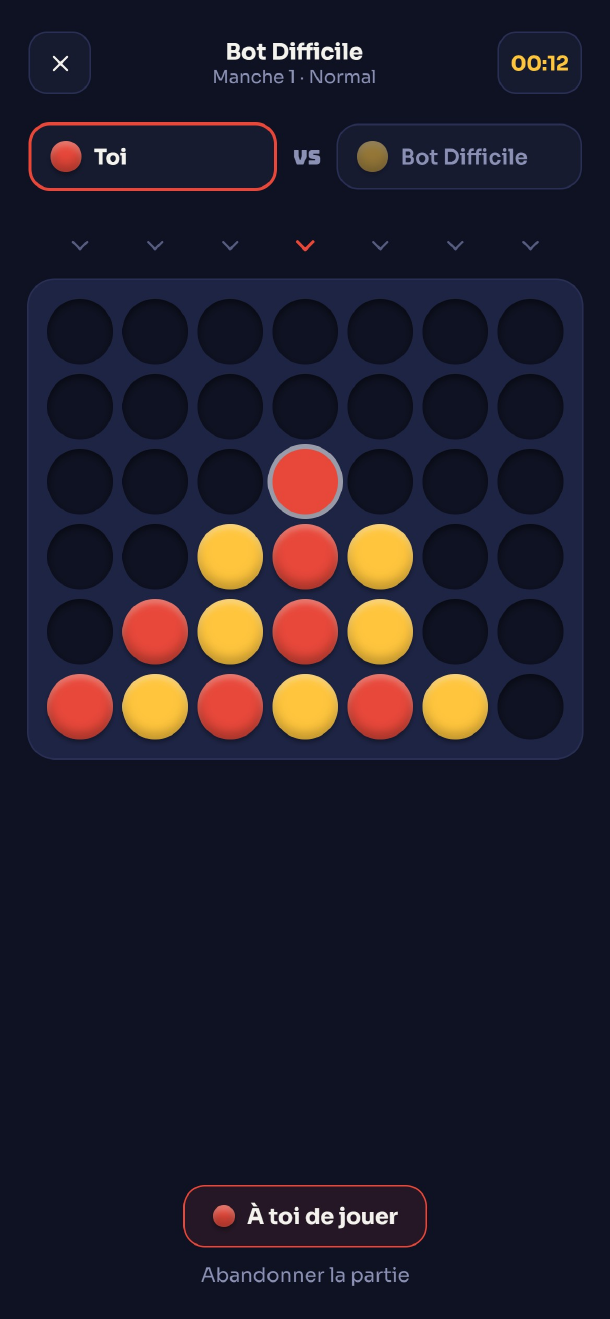
\includegraphics[width=\linewidth]{figures/maquette-8.png}\\[2pt]
\footnotesize (g) Écran de jeu
\end{minipage}
\caption{Maquettes de l'application}
\end{figure}

\textit{Les maquettes montrent 4 niveaux de bot à titre d'illustration ; l'application
en propose 3, tous basés sur des modèles RL.}

\end{document}
